%  LaTeX support: latex@mdpi.com
%  In case you need support, please attach any log files that you could have, and specify the details of your LaTeX setup (which operating system and LaTeX version / tools you are using).

%=================================================================

% LaTeX Class File and Rendering Mode (choose one)
% You will need to save the "mdpi.cls" and "mdpi.bst" files into the same folder as this template file.

%=================================================================

\documentclass[journal,article,accept,moreauthors,pdftex,12pt,a4paper,energies]{mdpi} 
%--------------------
% Class Options:
%--------------------
% journal
%----------
% Choose between the following MDPI journals:
% actuators, administrativesciences, aerospace, agriculture, agronomy, algorithms, animals, antibiotics, antibodies, antioxidants, appliedsciences, arts, atmosphere, atoms, axioms, behavioralsciences, bioengineering, biology, biomedicines, biomolecules, biosensors, brainsciences, buildings, cancers, catalysts, cells, challenges, chemosensors, children, chromatography, climate, coatings, computation, computers, cosmetics, crystals, dentistryjournal, diagnostics, diseases, diversity, econometrics, economies, education, electronics, energies, entropy, environmentalsciences, environments, fibers, foods, forests, futureinternet, galaxies, games, genes, geosciences, healthcare, humanities, informatics, information, inorganics, insects, ijerph, ijfs, ijms, ijgi, jcdd, jcm, jdb, jfb, joi, jlpea, jmse, jpcg, jpm, jrfm, jsan, land, laws, life, lubricants, machines, marinedrugs, materials, mathematics, medicalsciences, membranes, metabolites, metals, microarrays, micromachines, microorganisms, minerals, molbank, molecules, nanomaterials, ncrna, nutrients, pathogens, pharmaceuticals, pharmaceutics, pharmacy, photonics, plants, polymers, processes, proteomes, publications, religions, remotesensing, resources, risks, robotics, sensors, socialsciences, societies, sports, sustainability, symmetry, systems, technologies, toxics, toxins, vaccines, veterinarysciences, viruses, water
%---------
% article
%---------
% The default type of manuscript is article, but could be replaced by using one of the class options: 
% article, review, communication, commentary, bookreview, correction, addendum, editorial, changes, supfile, casereport, comment, conceptpaper, conferencereport, meetingreport, discussion, essay, letter, newbookreceived, opinion, projectreport, reply, retraction, shortnote, technicalnote, creative
%----------
% submit
%----------
% The class option "submit" will be changed to "accept" by the Editorial Office when the paper is accepted. This will only make changes to the frontpage (e.g. the logo of the journal will get visible), the headings, and the copyright information. Journal info and pagination for accepted papers will also be assigned by the Editorial Office.
% Please insert a blank line is before and after all equation and eqnarray environments to ensure proper line numbering when option submit is chosen
%------------------
% moreauthors
%------------------
% If there is only one author the class option oneauthor should be used. Otherwise use the class option moreauthors.
%---------
% pdftex
%---------
% The option "pdftex" is for use with pdfLaTeX only. If eps figure are used, use the optioin "dvipdfm", with LaTeX and dvi2pdf only.

%=================================================================
\setcounter{page}{1}
\lastpage{x}
\doinum{10.3390/------}
\pubvolume{xx}
\pubyear{2014}
\history{Received: xx / Accepted: xx / Published: xx}
%------------------------------------------------------------------
% The following line should be uncommented if the LaTeX file is uploaded to arXiv.org
%\pdfoutput=1

%=================================================================

% Add packages and commands to include here
% The amsmath, amsthm, amssymb, hyperref, caption, float and color packages are loaded by the MDPI class.
\usepackage{epstopdf}
\usepackage{graphicx}
\usepackage{subfigure}
\usepackage{tabularx}
\usepackage{multirow}
\usepackage{booktabs} 
\usepackage{soul}
%\newcommand{\hl}[1]{\textcolor{red}{\texttt{#1}}}

\providecommand{\sectionname}{Section}
\providecommand{\assignmentname}{Exercise}
\providecommand{\equationname}{Equation}
\providecommand{\figurename}{Fig\slashure}
\providecommand{\tablename}{Table}
\newcommand{\reffig}[1]{\normalsize\figurename~\ref{#1}\normalsize}
\newcommand{\reftab}[1]{\tablename~\ref{#1}}
\newcommand{\reflst}[1]{\lstlistingname~\ref{#1}}
\newcommand{\refchap}[1]{\chaptername~\ref{#1}}
\newcommand{\refapp}[1]{\appendixname~\ref{#1}}
\newcommand{\refsec}[1]{\sectionname~\ref{#1}}
\newcommand{\refeq}[1]{\equationname~\ref{#1}}
\newcommand{\refpage}[1]{on page~\pageref{#1}}



%=================================================================
%% Please use the following mathematics environments:
%\theoremstyle{mdpi}
%\newcounter{thm}
%\setcounter{thm}{0}
%\newcounter{ex}
%\setcounter{ex}{0}
%\newcounter{re}
%\setcounter{re}{0}
%\newtheorem{Theorem}[thm]{Theorem}
%\newtheorem{Lemma}[thm]{Lemma}
%\newtheorem{Characterization}[thm]{Characterization}
%\newtheorem{Proposition}[thm]{Proposition}
%\newtheorem{Property}[thm]{Property}
%\newtheorem{Problem}[thm]{Problem}
%\newtheorem{Example}[ex]{Example}
%\newtheorem{Remark}[re]{Remark}
%\newtheorem{Corollary}[thm]{Corollary}
%\newtheorem{Definition}[thm]{Definition}
%% For proofs, please use the proof environment (the amsthm package is loaded by the MDPI class).

%=================================================================

% Full title of the paper (Capitalized)
\Title{Shadow Replication: An Energy-Aware, Fault-Tolerant Computational Model for Green Cloud Computing}

% Authors (Add full first names)
\Author{Xiaolong Cui$^{1}$, Bryan Mills$^{1}$, Taieb Znati$^{1}$*, and Rami Melhem$^{1}$ }

% Affiliations / Addresses (Add [1] after \address if there is only one affiliation.)
\address{%
$^{1}$ Department of Computer Science, University of Pittsburgh\\
}

% Contact information of the corresponding author (Add [2] after \corres if there are more than one corresponding author.)
\corres{znati@cs.pitt.edu}

% Abstract (Do not use inserted blank lines, i.e. \\) 
\abstract{With the concerted efforts from researchers in hardware, software, algorithm, and data management, HPC is moving towards extreme-scale, featuring a computing capability of quintillion ($10^{18}$) FLOPS. 
As we approach the new era of computing, however, several daunting scalability challenges remain to be conquered. Delivering extreme-scale performance will require a computing platform that supports billion-way parallelism, necessitating a dramatic increase in the number of computing, storage, and networking components. At such a large scale, failure would become a norm rather than an exception, driving the system to significantly lower efficiency with unprecedented amount of power consumption. %The frequency and diversity of failures,  as well as the challenge of power, call for rethinking of the fault tolerance problem. 

To tackle this challeng, we propose an adaptive and power-aware algorithm, referred to as Lazy Shadowing, as an efficient and scalable approach to achieve high-levels of resilience, through forward progress, in extreme-scale, failure-prone computing environments. 
Lazy Shadowing associates with each process a ``shadow" (process) that executes at a reduced rate, and opportunistically rolls forward each shadow to catch up with the its leading process during failure recovery.
%overlaps the recovery time after each failure with the time needed to roll forward the shadows to a consistent state.
Compared to existing fault tolerance methods, our approach can achieve 20\% energy saving with potential reduction in solution time at scale.
}

% Keywords: add 3 to 10 keywords
\keyword{shadow computing; fault tolerance; scheduling; resilience; energy-aware}

% The fields PACS, MSC, and JEL may be left empty or commented out if not applicable
%\PACS{}
%\MSC{}
%\JEL{}

\begin{document}

%%%%%%%%%%%%%%%%%%%%%%%%%%%%%%%%%%%%%%%%%%

\section{Introduction}
\label{sec:introduction}
\noindent 
Cloud Computing has emerged as an attractive platform for increasingly
diverse compute- and data-intensive applications, as it allows for
low-entry costs, on demand resource provisioning and allocation and
reduced cost of maintaining internal IT
infrastructure~\cite{tchana_cits_2012}. Cloud computing will continue
to grow and attract attention from commercial and public market
segments. Recent studies predict annual growth rate of 17.7 percent by
2016, making cloud computing the fastest growing segment in the
software industry.

In its basic form, a cloud computing infrastructure is a large cluster
of interconnected back-end servers hosted in a datacenter and
provisioned to deliver on-demand, "pay-as-you-go" services and
computing resources to customers through a front-end
interface~\cite{ec2_site}. As the demand for cloud computing
accelerates, cloud service providers (CSPs) will be faced with the
need to expand their underlying infrastructure to ensure the expected
levels of performance, reliability and cost-effectiveness, resulting
in a multifold increase in the number of computing, storage and
communication components in their datacenters. The direct implication of large datacenters is increased management complexity and propensity to
failure. While the likelihood of a server failure is very small, the
sheer number of computing, storage and communications components that
can fail, however, is daunting. At such a large scale, failure becomes
the norm rather than an exception~\cite{schroeder_2010_dsc}.

As the number of users delegating their computing tasks to CSPs
increases, Service Level Agreements (SLAs) become a critical aspect
for a sustainable cloud computing business model. In its basic form,
an SLA is a contract between the CSPs and consumers that specifies the
terms and conditions under which the service is to be provided,
including expected response time and reliability. Failure to deliver
the service as specified in the SLA subjects the CSP to pay a penalty,
resulting in a loss of revenue.

In addition to penalties resulting from failure to meet the SLA
requirement, CSPs face rising energy costs of their large-scale
datacenters.  It is reported that energy costs alone could account
for 23-50\% of the expenses~\cite{Elnozahy03energyconservation} and
this bill mounts up to \$30 billion
worldwide~\cite{Raghavendra:2008:NPS}. This raises the question of how
fault tolerance might impact power consumption and ultimately the
expected profit of the service providers.

Current fault tolerance approaches rely upon either time or hardware
redundancy in order to tolerate failure. The first approach, which
uses time redundancy, requires the re-execution of the failed task
after the failure is detected.  Although this can further be optimized
by the use of checkpointing and roll-back recovery, such an approach
can result in a significant delay increase subjecting CSPs to penalties, when SLA terms are violated,
and high energy costs due to re-execution of failing tasks.

%, with two consequences on
%profit. First, the CSP may be subjected to paying a penalty to the
%customer for failure to deliver the expected service within the
%negotiated time constraints. Second, the need to re-execute the
%failed task increases energy consumption.


The second approach exploits hardware redundancy and executes multiple
instances of the same task in parallel to overcome failure and
guarantee that at least one task reaches completion.  This approach,
which has been used extensively to deal with failure in critical
applications, is currently used in cloud-computing to provide fault
tolerance while hiding the delay of
re-execution~\cite{tsai_isads_2011,ko_socc_2010}. This solution,
however, increases the energy consumption for a given service, which
in turn might outweigh the profit gained by providing the service.
The trade-off between profit and fault-tolerance calls for new
frameworks to take both SLA requirements and energy awareness in
dealing with failures.

In this paper, we address the above trade-off challenge and propose an
energy-aware, SLA-based profit maximization framework, referred to as
``Shadow Replication'', for resilience in cloud computing.  Similar to
traditional replication, Shadow Replication ensures successful task
completion by concurrently running multiple instances of the same
task. Contrary to traditional replication, however, Shadow Replication
executes the main instance of the task at the speed required to
maximize profit and uses dynamic voltage and frequency scaling (DVFS)
to slow down the execution of the replicas, thereby enabling a
parameterized trade-off between response time, energy consumption and
hardware redundancy. This allows CSPs to maximize the expected profit
by accounting for income, potential penalties and energy cost.

%the
%basic idea of shadow replication is to ensure the completion of a task
%by concurrently running multiple replicas of a process, but in a much
%smarter way: it provides fault tolerance by combining replication with
%dynamic voltage and frequency scaling (DVFS), enabling a parameterized
%tradeoff between time and hardware redundancy.

The main challenge of Shadow Replication resides in determining
jointly the execution speeds of all task instances, both before and
after a failure occurs, with the objective to minimize energy and
maximize profit.  In this paper, we propose a reward-based analytical
framework to achieve this objective. The main contributions of this paper
are as follows:

\begin{itemize}
%\item A profit-based optimization framework to compute the different speeds of %formalization of shadow replication as 
%\item The use of Shadow Replication to maximize the economic potential
%  of cloud computing.

\item An energy-aware, SLA-based, profit maximization execution model, referred to as
``Shadow Replication'', for resilient cloud computing.

\item A profit-based optimization model to explore the applicability of
  Shadow Replication to cloud computing, and to determine the optimal
  speeds of all task instances to maximize profit.

\item In environments where either the specification or
the detection of failure is hard to achieve, we propose a sub-optimal,
yet practical resilience scheme, called profit-aware stretched
replication.

\item An evaluation framework to analyze profit and 
energy savings achievable by Shadow Replication, compared to existing resilience methods.
%including a
%comparative analysis of the different resilience methods, to identify
%the most profitable technique for various computing environments.

%\item An analysis of the profit gain and energy savings achievable by
 % using shadow replication.
%\item A comparative analysis of the different resilience methods, including pure %replication and re-execution, and identification 
 % of the most profitable technique for a given system configuration and failure %rate.
\end{itemize}

%The analysis shows that in all cases, shadow replication outperforms
%traditional replication. Furthermore, the results show that shadow
%replication is the most efficient fault tolerance method when the rate
%of system failure is high. It is also observed that when the target
%response time is stringent, shadow replication converges to
%traditional replication, as expected.

The analysis shows that in all cases, Shadow Replication outperforms
existing fault tolerance methods. Furthermore, shadow
replication would converge to traditional replication, when target response time is stringent, and to re-execution when target response time is relaxed or failure is unlikely, as expected.

The rest of the paper is organized as follows. We begin by describing a
computing model typically used in cloud computing for compute- and
data-intensive applications in
Section \ref{sec:cloud_computing_workload}. We then introduce
the Shadow Replication framework in
Section \ref{sec:shadow_replication}. Section
\ref{sec:reward_model},  \ref{sec:reward_model_2}, and \ref{sec:reward_model_3} present our analytical models and optimization
problem formalization, followed by experiments and evaluation in
section \ref{sec:evaluation}. Section \ref{sec:related_work} briefly
surveys related work. Section \ref{sec:conclusion} concludes this work.



\section{Cloud Workload Characterization}
\label{sec:cloud_computing_workload}
%\noindent 

Today's popular online services, such as web search, video streaming,
and social networks, are all powered by large data centers. In
addition to these public services, high-performance applications and
business activities are migrating onto cloud computing~\cite{Ferdman:2012:CCS:2150976.2150982,mrbs}. Table \ref{tbl:apps}
lists several classes of cloud computing applications. 

\begin{table}[!h]
	\caption{Typical cloud computing applications.}
	\centering
		\begin{tabularx}{\columnwidth}{|l|X|}
			\hline
			Class                          & Examples                         \\
			\hline
			Data Analytics   & Bioinformatics\\ 
			& Business Intelligence\\
			\hline
			Graph Analytics  & Social Networks\\ 
			& Recommendation Systems\\
			\hline
			Web Search       & Text Processing\\
			& Recommendation Systems\\
			\hline
			\end{tabularx}
	\label{tbl:apps}
\end{table}

Two main characteristics of the above applications are large dataload
and high parallelism. In 2008, Google processed 20 PB of data with
MapReduce each day; in April 2009, a blog revealed eBay's 2 enormous
data warehouses: one with 2 PB of data and the other with 6.5 PB of
data; shortly thereafter, Facebook announced that a 2.5
Peta-bytes of user data, at a growth rate of at 15 Tera-bytes per day~\cite{lin2010data}. 
Without massive parallelism, handling such volumes of data is beyond the processing capability of curent computing infrastructre. 

Each job, that involves processes these data, typically requires multiple
phases that execute in sequence. During each phase, workload is
splited into tasks and processed in parallel to speed up the whole
process.  Consequently, a cloud computing job can be modeled as 
a set of tasks, executing in parallel on different computing nodes. For the job to complete, all tasks must finish their exectution. 
Consequently, if a task is delayed then all remaining tasks must wait, until the delayed task completes. 
This model is directly reflective of the \emph{MapReduce}
computational model, which is predominately used in Cloud
Computing \cite{mrbs}.  

Each job has a targeted response time defined
by the terms of the SLA. Further, the SLA defines the amount to be
paid for completing the job by the targeted response time as well as
the penalty to be incurred if the targeted response time is not
met. 

Each task is mapped to one compute core and executes at a speed, $\sigma$. The partition of the job among tasks is
such that each task processes a similar
workload, $W$. Consequently, baring failures, tasks are expected to
complete at about the same time. Therefore, the minimal response time
of each task, when no failure occurs, is
$t_{min}~=~\frac{W}{\sigma_{max}}$, where $\sigma_{max}$ is the maximum speed. This is also the minimal response
time of the entire phase. 

As the number of tasks increases, however, the likelihood of a task
failure during an execution of a given phase increases
accordingly. This underscores the importance of an energy-efficient
fault-tolerance model to mitigate the impact of a failing task on the
overall delay of the execution phase. The following section describes
Shadow Replication, a fault-tolerant, energy-aware computational model to achieve profit-maximizing resiliency in cloud computing.


\section{Shadow Replication}
\label{sec:shadow_replication}
\begin{figure*}[!t]
	\begin{center}
		\subfigure[No Failure]
		{
			\label{fig:sc_no_fail}
			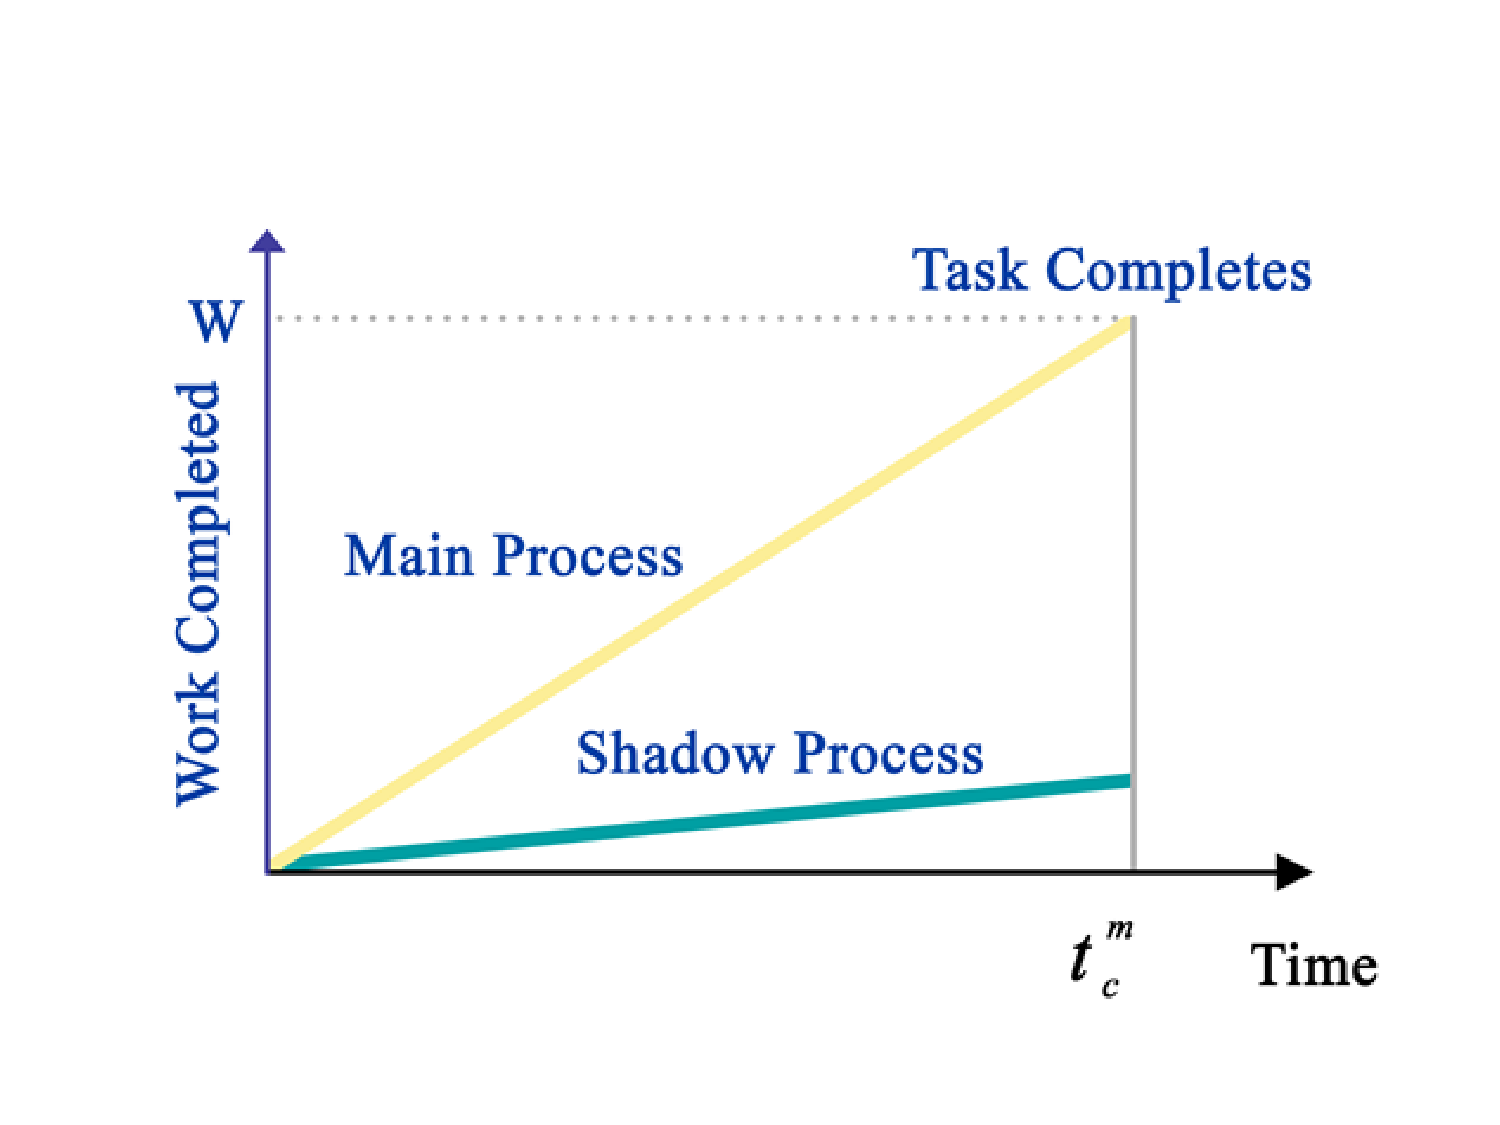
\includegraphics[width=0.32\textwidth]{diagrams/example1.pdf}
		}
		\subfigure[Shadow Process Failure]
		{
			\label{fig:sc_shadow_fail}
			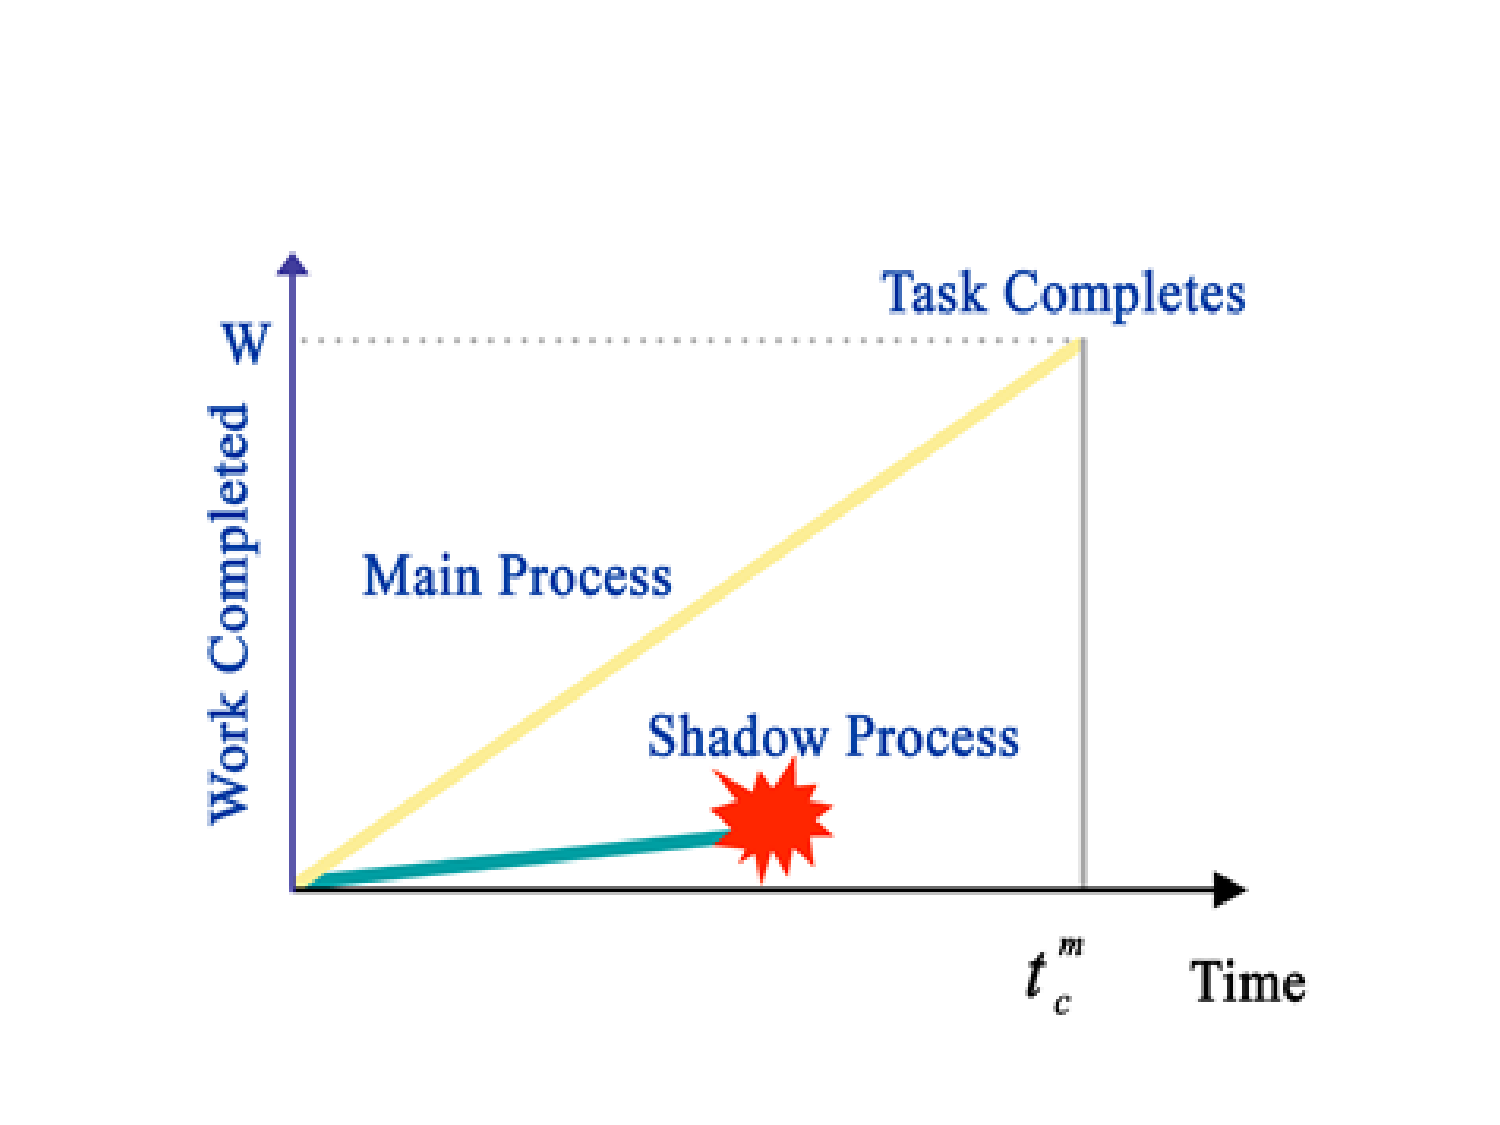
\includegraphics[width=0.29\textwidth]{diagrams/example3.pdf}
		}
		\subfigure[Main Process Failure]
		{
			\label{fig:sc_main_fail}
			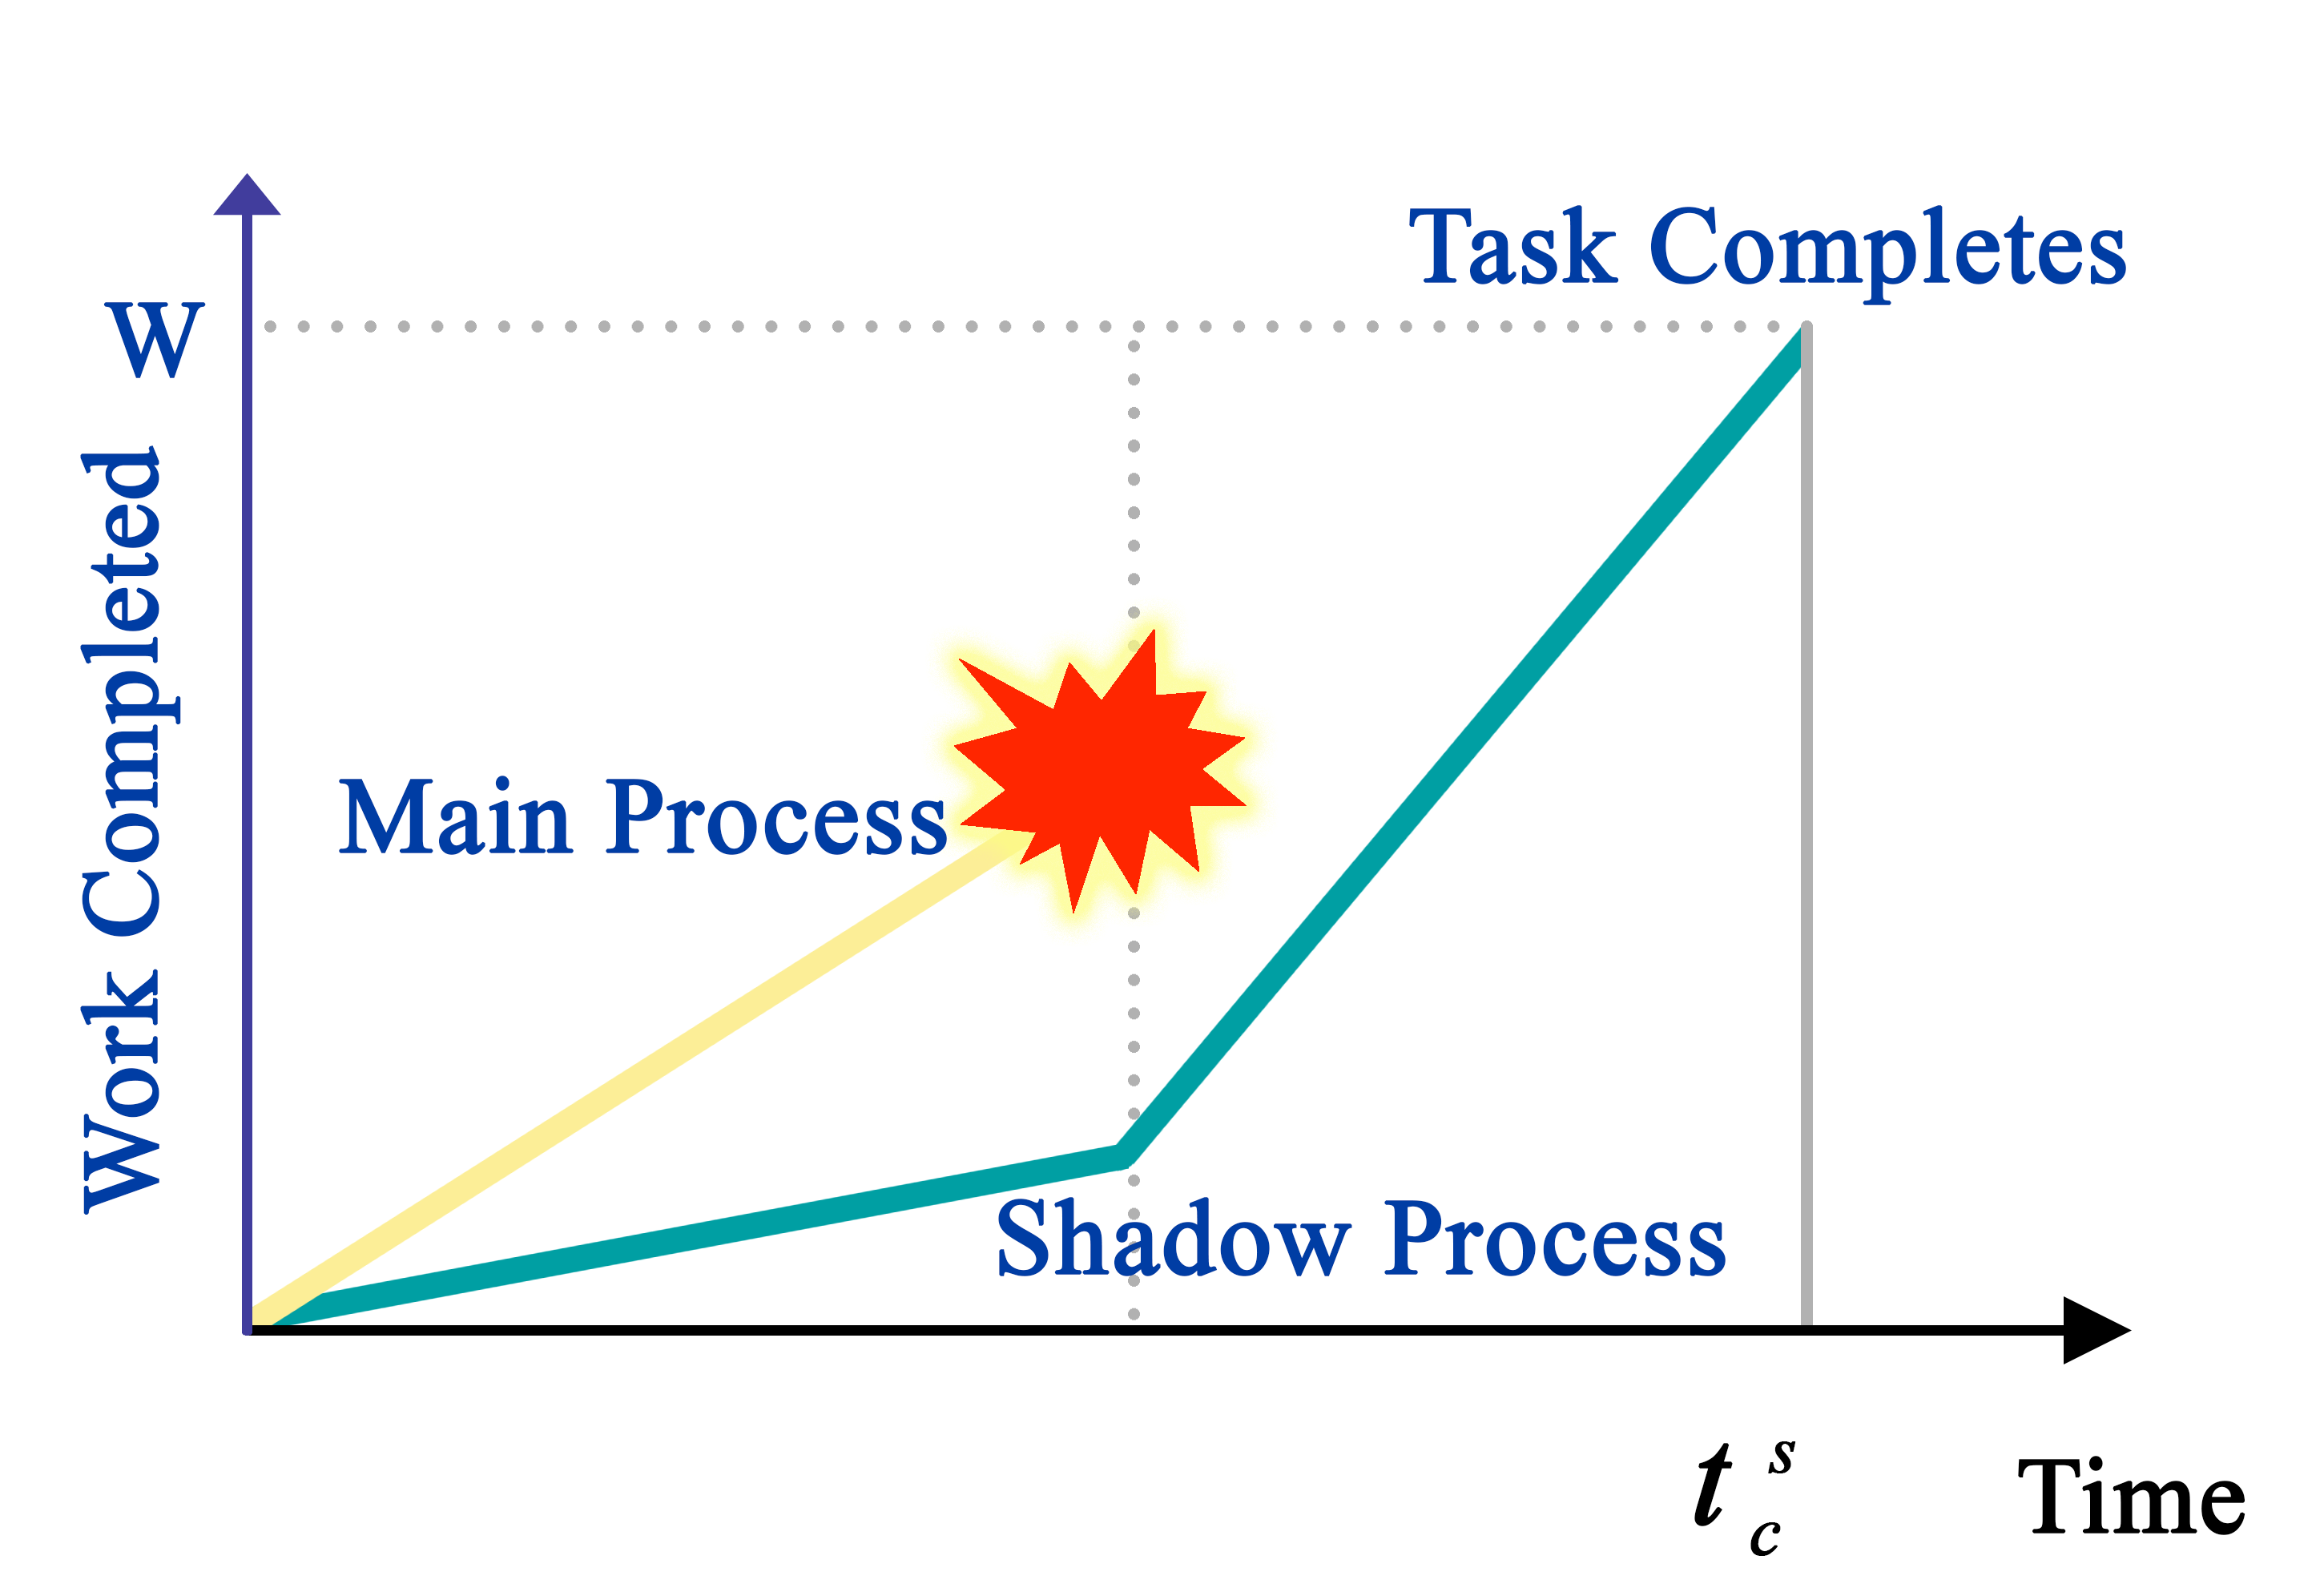
\includegraphics[width=0.33\textwidth]{diagrams/example2.png}
		}
	\end{center}
	\caption{Shadow replication for a single task and single replica}
	\label{fig:sc_overview}
\end{figure*}

\noindent 
The basic tenet of Shadow Replication is to associate with each
main process a suite of ``shadows'' whose size depends on the
``criticality'' of the application and its performance requirements,
as defined by the SLA. 
%To overcome potential failures, the shadows
%execute on separate computing nodes, concurrently with but at slower
%speeds than, the main process.

%The successful completion of the main
%process results in the immediate termination of all shadow
%processes. If the main process fails, the primary shadow process takes
%over the role of the main process and resumes computation, possibly at
%an increased speed, in order to complete the task at a targeted
%response time.


Formally, we define the Shadow Replication fault-tolerance model as follows:
\begin{itemize}
\item A main process, $P_m(W,\text{ }\sigma_m)$, whose responsibility is to executes a task of size $W$ at a speed of $\sigma_m$;
\item A suite of shadow processes, $P_{s}(W,\text{ }\sigma_b^s, \text{ }\sigma_a^s)$ ($1 \le s \le \cal S)$, where $\cal S$ is the size of the suite. 
The shadows execute on separate computing nodes. Each shadow process is associated with two execution speeds. All shadows start execution simultaneously with the main process at speed $\sigma_b^s$ ($1 \le s \le \cal S$). Upon failure of the main process, all shadows switch their executions to $\sigma_a^s$, with one shadow being designated as the new main process. This process continues until completion of the task.
\end{itemize}
%All shadows execute simultaneously with the main process at speed $\sigma_a^s$

To illustrate the behavior of Shadow Replication, we limit the number of shadows to a single process and consider the scenarios depicted in Figure \ref{fig:sc_overview}, assuming a single process failure. Figure \ref{fig:sc_no_fail} represents the case when neither the main nor the shadow fails. The main process, executing
at a higher speed, completes the task at time $t_c^m$. At this time, the shadow process, progressing at a lower speed, stops execution immediately. Figure \ref{fig:sc_shadow_fail} represents the case when the shadow fails. This failure, however, has no impact on the progress of the main process, which still completes the task at $t_c^m$. Figure \ref{fig:sc_main_fail} depicts the case when the main process fails while the shadow is in progress. After detecting the failure of the main process, the shadow begins execution at a higher speed, completing the task at time $t_c^s$. When possible, the shadow execution speed upon failure must be set so that $t_c^s$ does not exceed $t_c^m$. Given that the failure rate of an individual node is much lower than
the aggregate system failure, it is very likely that the main process
will always complete its execution successfully, thereby achieving fault tolerance at a significantly reduced cost of energy consumed by the shadow. %saving a lot of energy for its associated shadow processes. 

%In summary, shadow replication has the following characteristics:
%The proposed shadow replication model has several properties:
%\begin{itemize}
%\item The main process is associated with only one execution speed, $\sigma_m$, %which depends on the size of the task and the SLA requirement.
%\item The shadow processes execute with two different speeds, which are failure %dependent and when possible should be computed to meet the SLA requirement as %closely as possible. 
%\item The completion of the main process results in the immediate termination of %all shadow processes. Given that the failure rate of an individual node is much %lower than the aggregate system failure, it is very likely that the main process %completes successfully, saving a significant amount of energy, while achieving %high level of fault tolerance.
%\end{itemize}



A closer look at the model reveals that shadow
replication is a generalization of traditional fault tolerance
techniques, namely re-execution and traditional replication. If the
SLA specification allows for flexible completion time, shadow
replication would take advantage of the delay laxity to trade time
redundancy for energy savings. It is clear, therefore, that for a
large response time, Shadow Replication converges to re-execution, as
the shadow remains idle during the execution of the main process and
only starts execution upon failure. If the target response time is
stringent, however, Shadow Replication converges to pure replication,
as the shadow must execute simultaneously with the main at the same
speed. The flexibility of the Shadow Replication model provides the
basis for the design of a fault tolerance strategy that strikes a
balance between task completion time and energy saving, thereby
maximizing profit.

Given that the probability of two individual nodes executing the same
instances of a task fail at the same time is low, we will focus on the study of Shadow Replication model with a single shadow. It is clear, however, that the model can
be extended to support multiple processes, as required by the
application's fault-tolerance requirement. Furthermore, we adopt the
fail-stop~ fault model, where a processor stops execution once a fault
occurs and failure can be detected by other
processes\cite{gartner_faults_1999,cristian_comm_1991}.

%While all
%shadow processes are exact replicas of the main process, one among
%these processes, referred to as primary shadow process, is special in
%that it would become new main process if current one fails.

% stated in paragraph one now.
%In order to mask failure during a task,
%the shadow processes are scheduled to execute concurrently with the
%main process, but on different computing nodes. Furthermore, in order
%to reduce energy, shadow processes initially execute at decreasingly
%lower processor speeds.


%Moreover, one among the remaining shadow processes is promoted
%to primary shadow process. By allowing instantaneous fail-over with
%shadow processes in the event of failure, shadow replication eliminates
%even the smallest chance of data loss or disruption.


%Without loss of generality, from this point on we
%assume at most one failure would occur to a task and consider a dual
%level of redundancy, whereby only one shadow process is executed
%concurrently with each main process. The completion of the main or its
%shadow results in the successful execution of the task. If the main
%process fails, it is implied that shadow process would complete the
%task.



% needless words
%Figure \ref{fig:sc_overview} depicts how shadow replication works to
%complete a single task using a single replica. While the main process
%would execute at a certain fixed speed until task completion or
%failure, the shadow process may change its speed if it needs to take
%over the role of main process, in order to finish task in
%time. According to if and when failure occurs, there are three cases
%that may happen during the execution of the task.


%In this section we have defined shadow replication and described its
%potential in energy saving and profit gain in cloud computing
%environment. Three questions, however, remain to be answered before we
%expect shadow replication to be accepted as a novel fault tolerance
%technique for cloud computing: 1) is it truly possible for shadow
%computing to save energy and bring more profit over state-of-the-art
%fault tolerance approaches while meeting SLA requirements; 2) if so,
%how much benefit can it bring; 3) how to determine the optimal
%execution speeds for main process and shadow processes.
%
%To answer the above questions, in the following section we will
%introduce a reward-based analytical model for fault tolerance
%mechanisms with a dual-level redundancy under the assumption that at
%most one process may fail.


%\section{\uppercase{Resilient Methods}}
%\label{sec:resilient_methods}
%There are two main ways of handling task failures, re-execution or
replication. In the next section we will define these resilience
methods and introduce two new profit-optimized replication schemes.

\subsection{Re-execution}

Re-execution simply re-executes the task when a failure occurs until
the task completes successfully. This will result in delaying the job
completion because all tasks must complete in order to complete the
job. This will impact profit in at least two directions, first the
delay might result in the service provider paying a penelty to the
client and secondly it might result in increased energy consumption
because of the extended execution time.

\subsection{Traditional Replication}

Traditional replication is a method in which each task is replicated
on independent computing nodes, such that if one process fails its
replica process can continue executing as if the failure did not
occur. This is also referred to as process replication and has long
been deployed in mission critical applications. Replication has been
used extensively in cloud computing
\cite{tsai_isads_2011,ko_socc_2010} but is often criticized in
task-based jobs because of the use of additional resources. From a
profit standpoint this will reduce the liklihood of paying a penelty
under the SLA but could significanlly increase the energy consumption.

\subsection{Profit-aware Replication}

Service providers want to maximize their revenue and reduce their
expenses, in the next sections we will introduce two profit-optimized
resilience methods. These methods seek to strike a balance between
energy consumption and revenue obtained under the terms of the SLA.

\subsubsection{Optimized Stretched Replication}

Stretched replication works on the assumption that performing work
slowly can save energy. This is typically done through the use of
dynamic voltage and frequency scaling (DVFS). Stretched replication
slows down the execution of all processes to the slowest possible
speed while maximizing the profit. As we will show in detail in
Section \ref{sec:stretched_replication_model}, this optimization
accounts for the energy cost and the terms dictated in the SLA.

\hl{The only reason I can think this is a good idea is if error
  detection is expensive. This would be an argument for presenting
  shadow computing first then introduce this as a modiciation if error
  detection is hard or impossible. I didn't do it this way but think
  it might be a better way after discussing with Taieb.}

\subsubsection{Optimized Shadow Replication}

\input{shadow_computing}



\section{Reward Based Optimal shadow replication}
\label{sec:reward_model}
\noindent 

In this section, we describe a profit-based optimization framework for
the cloud-computing execution model previously described. 
In this framework, we adopt the fail-stop fault model, where a processor stops execution once a fault
occurs and failure can be detected by other processes\cite{gartner_faults_1999,cristian_comm_1991}.
Furthermore, given that the probability of two individual nodes executing the same
instances of a task fail at the same time is low, we will focus on the study of Shadow Replication model with a single shadow.
Consequently, the completion of the main or its shadow results in the successful execution of the task. If the main
process fails, it is implied that shadow process would complete the
task.  It is clear, however, that the model can
be extended to support multiple shadow processes, as required by the
application's fault-tolerance requirement. 

Using this
framework we compute profit-optimized execution speeds by
optimizing the following objective function:

%It is assumed that failures can be detected.

%While this is the case in many computing
%environments, there are cases where failure detection may not be
%possible. To address this limitation, we propose a sub-optimal shadow
%replication scheme, whereby both the main process and the shadow
%execute independently at stretched speeds to meet the expected
%response time, without the need for the main processes failure
%detection.

%In this section, we describe a reward-based analytical
%model to guide the design of the shadow replication scheme that
%executes at optimal speed to maximize profits. 


%In this section we are going to develop a framework to assess and
%explore the trade-off between energy consumption and performance of
%fault tolerant computation models, namely shadow replication, pure
%replication, and re-execution. To this end, we adopt a reward-based
%model to study the economic potential of shadow replication, analyze its
%interplay between resiliency and power management, and compare it to
%other fault tolerance models.

%Without loss of generality, we focus on the execution of one job as
%shown in Fig. 2, assuming that there are N tasks in total that will
%execute in parallel. The completion of the job depends on the
%successful execution of all these tasks, and a failure in one task
%would delay the completion of the entire job.

\begin{equation}
\label{optimization_problem}
%\setlength{\abovedisplayskip}{14pt}
\begin{alignedat}{2}
\max_{\sigma_m,\sigma_b,\sigma_a}     & E[profit] \\
s.t.                                 & 0 \leq \sigma_m \leq \sigma_{max} \\
                                     & 0 \leq \sigma_b \leq \sigma_{m} \\
                                     & 0 \leq \sigma_a \leq \sigma_{max} 
\end{alignedat}
\end{equation}
We assume that processor
speeds are continuous and use nonlinear optimization techniques
to solve the above optimization problem. 

In order to earn profit, service providers must either increase
income or decrease expenditure. We take both factors into
consideration for the purpose of maximizing profit while meeting
customer's requirements. In our model, we set the expected profit to be
expected income minus expected expense.

\begin{equation}
E[\text{profit}]=E[\text{income}]-E[\text{expense}]
\end{equation}

\subsection{Reward Model}
\label{sla_reward_model}
The cloud computing SLA can be diverse and
complex. To focus on the profit and reliability
aspects of the SLA, we define the reward model based on job completion
time. Platform as a Service (PaaS) companies will continue to become
more popular causing an increase in SLAs using job completion time as
their performance metric. We are already seeing this appear in
web-based remote procedure calls and data analytic requests.

As depicted in Figure \ref{fig:reward}, customers expect that their
job deployed on cloud finishes by a mean response time $t_{R_1}$.  As a
return, the provider earns a certain amount of reward, denoted by R,
for satisfying customer's requirements. However, if the job cannot be
completed by the expected response time, the provider loses a fraction of $R$
proportional to the delay incurred. For large delay, the profit loss may translate into a penalty that the CSP must pay to the customer. In this model, the maximum penalty $P$ is paid if the
delay reaches or exceeds $t_{R_2}$. The four
parameters, $R$, $P$, $t_{R_1}$ and
$t_{R_2}$, completely define the reward model.

%The three parameters, R, and should be determined while negotiating
%the SLA according to the task workload. In our model, R is
%proportional to the expected energy cost that SP has to pay for
%executing customer’s tasks. Especially, R can grow with workload in a
%linearly proportional manner, logarithmic manner, or exponential
%manner.
%
%, which
%should be larger than the minimal response time . 

There are two facts that the service provider must take into account
when negotiating the terms of the SLA. The first is the response time
of the main process assuming no failure (Figure
\ref{fig:sc_no_fail} and Figure \ref{fig:sc_shadow_fail}). This
results in the following completion time:
\begin{equation}
t_c^m=W/\sigma_m
\label{eq:tcm}
\end{equation}

If the main process fails (shown in Figure \ref{fig:sc_main_fail}), the
task completion time by shadow process is the time of the failure,
$t_f$, plus the time necessary to complete the remaining work.

\begin{equation}
t_c^s=t_f+\frac{W-t_f \times \sigma_b}{\sigma_a}
\label{eq:tcs}
\end{equation}

This reward model is flexible and extensible; it is not restricted to
the form shown in Figure \ref{fig:reward}. In particular, the decrease
may be linear, concave, or convex and the penalty can extend to
infinity. This model can further be extended to take into
consideration both the short-term income and long-term reputation of
the service provider~\cite{Daw:2002:LRP:639717.639720}.


\begin{figure}[t!]	
	\begin{center}
		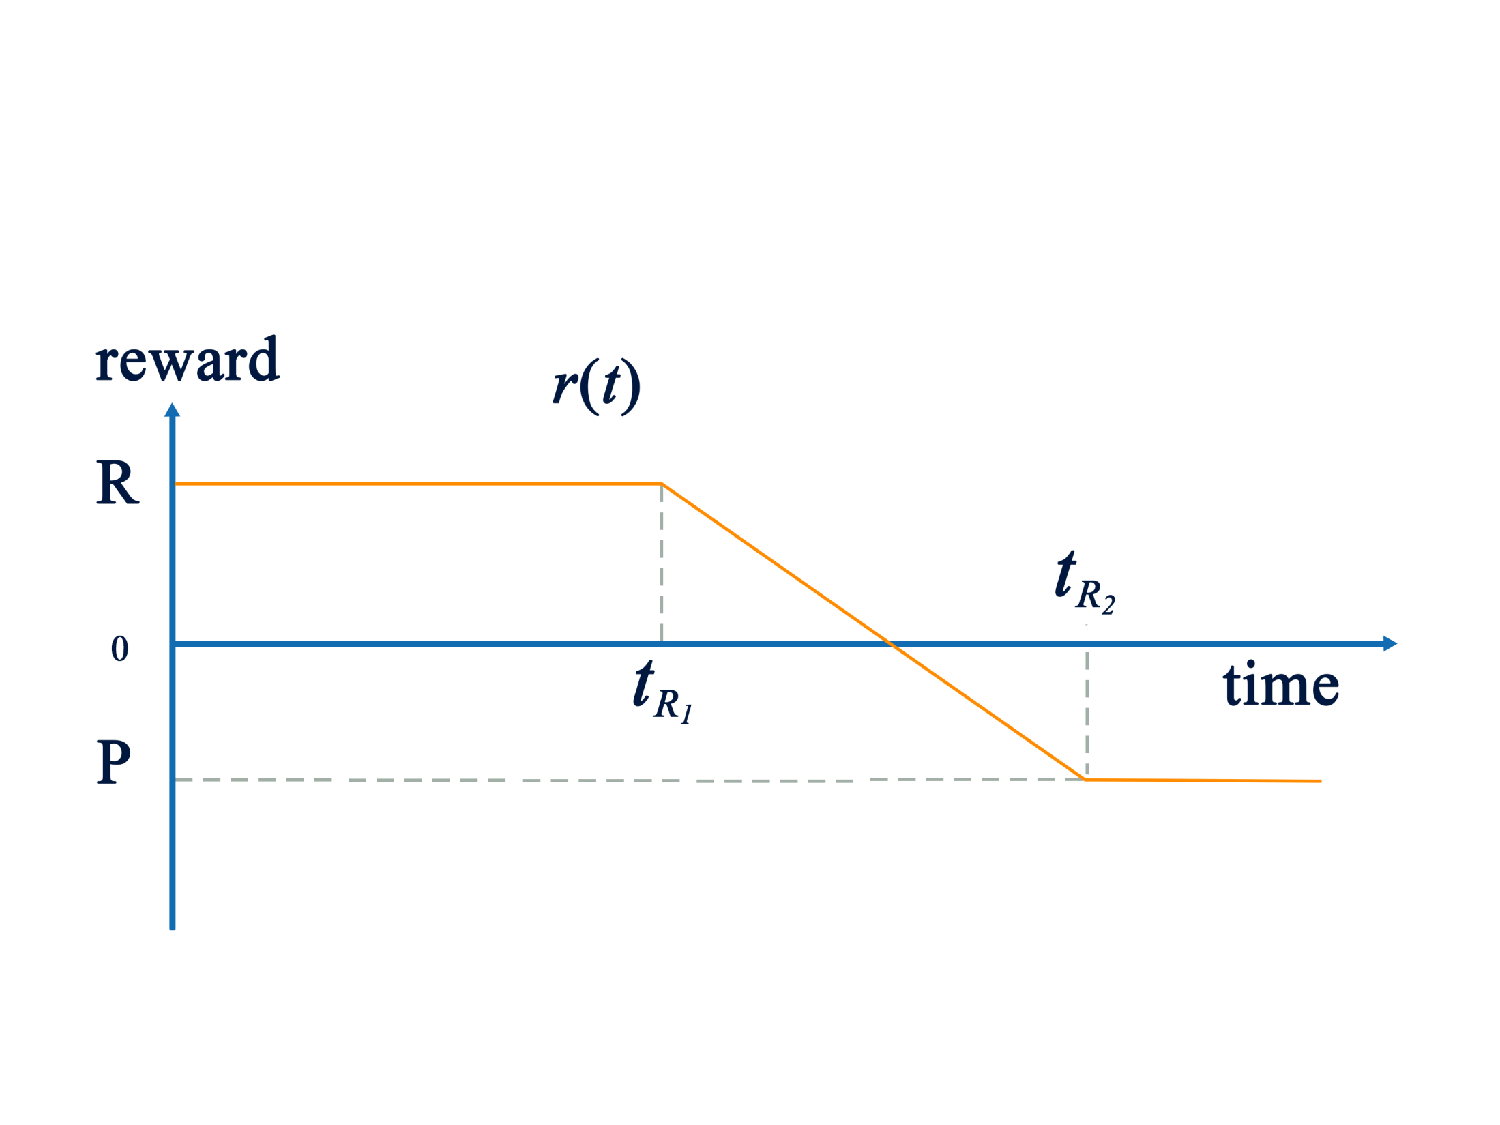
\includegraphics[width=\columnwidth]{diagrams/reward.pdf}
	\end{center}
	\caption{A reward function}
	\label{fig:reward}
\end{figure}


\subsection{Failure Model}
Failure can occur at any point during the execution of the main or
shadow process. Our assumption is that at most one failure occurs,
therefore if the main process fails it is implied that the shadow will
complete the task without failure. We can make this assumption because
we know the failure of any one node is rare thus the failure
of any two specific nodes is very unlikely.

% I don't think we need to say this and it opens us up to having to
% explain multiple shadows which we do not do today.
%In order
%to achieve higher resiliency one would make use of multiple shadow
%processes and this failure model will still be valid.

We assume that two probability density functions, $f_m(t_f)$ and
$f_s(t_f)$, exist which express the probabilities of the main and shadow
process failing at time $t_f$ separately. The model does not assume a
specific distribution. However, in the remainder of this paper we use
an exponential probability density function, $f_m(t_f)=f_s(t_f)=\lambda
e^{-\lambda t_f}$, of which the mean time between failure (MTBF) is $\frac{1}{\lambda}$.

\subsection{Power and Energy Models}
Dynamic voltage and frequency scaling
(DVFS) has
been widely exploited as a technique to reduce CPU dynamic power~\cite{flautner_2002_APS,pillai_2001_sosp}. It
is well known that one can reduce the dynamic CPU power consumption at
least quadratically by reducing the execution speed linearly. The
dynamic CPU power consumption of a computing node executing at speed
$\sigma$ is given by the function $p_d(\sigma)=\sigma^n$ where $n \ge
2$.
%% removed burd_1995_systems citation

In addition to the dynamic power, CPU leakage and other components
(memory, disk, network etc.) all contribute to static power
consumption, which is independent of the CPU speed. In this paper we
define static power as a fixed fraction of the node power consumed
when executing at maximum speed, referred to as $\rho$. Hence node
power consumption is expressed as
$p(\sigma)=\rho \times \sigma_{max}^n + (1-\rho)\times \sigma^n$. When the execution speed is zero
the machine is in a sleep state, powered off or not assigned as a
resource; therefore it will not be consuming any power, static or
dynamic.  Throughout this paper we assume that dynamic power is cubic
in relation to
speed~\cite{rusu_2003_ecs,zhai_2004_dac}, therefore the
overall system power when executing at speed $\sigma$ is defined as:
\begin{equation}
p(\sigma) = \begin{cases} \rho \sigma_{max}^3 + (1-\rho) \sigma^3 & \mbox{if } \sigma > 0 \\ 
                          0 & \mbox{if } \sigma = 0 \end{cases}
\label{eq:power_model}
\end{equation}
%% I removed chen_2012_srds from speed citation to save space

Using the power model given by \refeq{eq:power_model}, the
energy consumed by a process executing at speed $\sigma$ during an
interval $T$ is given by
\begin{equation}
E(\sigma,T) = p(\sigma) \times T
\end{equation}

%We derive the expected energy consumption of shadow replication for a
%single task assuming the failure model described
%previously. 

Corresponding to \reffig{fig:sc_overview}, there are three
failure cases to consider: main and shadow both succeed, shadow fails
and main fails. As described earlier, the case of both the main and
shadow failing is very rare and will be ignored. The expected
energy consumption for a single task is then the weighted average of
the expected energy consumption in the three cases.

%Each task is dependent upon the completion of all other tasks, this
%means that if a task completes prior to another task it must idly wait
%for that task to complete. In our system model a task will have to
%wait if at least one main process fails to complete, thus forcing all
%tasks to wait until the latest shadow process completes. 

First consider the case where no failure occurs and the main process
successfully completes the task at time $t_c^m$, corresponding to
\reffig{fig:sc_no_fail}.
\begin{equation}
\begin{split}
E_1 = &  ( 1-\int_0^{t_c^m}f_m(t)dt) \times (1 - \int_0^{t_c^m} f_s(t)dt) \times \\
      &  (  E(\sigma_m,t_c^m) + E(\sigma_b,t_c^m))
\label{eq:energy_no_failure}
\end{split}
\end{equation}
The first line is the probability of fault-free execution of the main
process and shadow process. Then we multiple this probablity by the
energy consumed by the main and the shadow process during this fault
free execution, ending at $t_c^m$.

Next, consider the case where the shadow process fails at some point
before the main process successfully completes the task, corresponding to
\reffig{fig:sc_shadow_fail}.
\begin{equation}
\begin{split}
E_2 = & (1-\int_0^{t_c^m}f_m(t)dt) \times \\
      & \int_0^{t_c^m}(E(\sigma_m,t_c^m)+E(\sigma_b,t)) \times f_s(t)dt
\label{eq:energy_shadow_fail}
\end{split}
\end{equation}
The first factor is the probability that the main process does not
fail, and the probability of shadow fails is included in the second factor which also contains the energy consumption since it depends on the shadow failure time. Energy consumption comes from the main process until the completion of the task,
and the shadow process before its failure.

The one remaining case to consider is when the main process fails and
the shadow process must continue to process until the task completes,
corresponding to Figure \ref{fig:sc_main_fail}.
\begin{equation}
\begin{split}
E_3 = & (1-\int_0^{t_c^m}f_s(t)dt) \times \int_0^{t_c^m}(E(\sigma_m,t)+\\
      & E(\sigma_b,t)+E(\sigma_a,t_c^s-t))f_m(t)dt
\label{eq:energy_main_fail}
\end{split}
\end{equation}
Similarly, the first factor expresses the probability that the shadow process does
not fail. In this case, the shadow process executes from the beginning to
$t_c^s$ when it completes the task. However, under our ``at most one
failure'' assumption, the period during which shadow process may fail
ends at $t_c^m$, since the only reason why shadow process is still in
execution after $t_c^m$ is that main process has already failed. There
are three parts of energy consumption, including that of main process
before main's failure, that of shadow process before main's failure,
and that of shadow process after main's failure, all of which depend
on the failure occurrence time. 

The three equations above describe the expected energy consumption by a
pair of main and shadow processes for completing a task under
different situations. However, under our system model it might be the
case that those processes that finish early will wait idly and
consume static power if failure delays one task. If it is the case
that processes must wait for all tasks to complete, then this energy
needs to be accounted for in our model. The probability of this is the probability that at least one main process fails,
referred to as the system level failure probability.
\begin{equation}
P_f=1-(1-\int_0^{t_c^m}f_m(t)dt)^N
\label{eq:prob_of_one_main_failure}
\end{equation}
Hence, we have the fourth equation corresponding to the energy consumed while waiting in idle. 
\begin{equation}
  \begin{split}
  E_4 = & ( 1-\int_0^{t_c^m}f_m(t)dt) \times (1 - \int_0^{t_c^m} f_s(t)dt) \times \\
        & 2 P_f \times E(0,t_c^j-t_c^m) + \int_0^{t_c^m}f_s(t)dt \times \\
        & (1-\int_0^{t_c^m}f_m(t)dt) \times P_f \times E(0,t_c^j-t_c^m) 
  \end{split}
\end{equation}
Corresponding to the first case, neither main process nor shadow
process fails, but both of them have to wait in idle from task
completion time $t_c^m$ to the last task's completion (by a shadow
process) with probability $P_f$. Under the second case, only the main
process has to wait if some other task is delayed since its shadow
process has already failed. These two aspects are accounted in the
first and last two lines in $E_4$ separately.  We use the expected
shadow completion time $t_c^j$ as an approximation of the latest task
completion time which is also the job completion time.

%% Rami said remove, I agree - bnm
%and the reason why we
%ignore the third case is that the third case itself accounts for the
%delayed task and it is already factored in $E_3$. 

%\begin{equation}
%t_c^j=\frac{\int_0^{t_c^m}t_c^s \times f_m(t)dt}{\int_0^{t_c^m}f_m(t)dt}
%\label{eq:estimated_shadow_completion}
%\end{equation}

By summing these four parts and then multiplying it by $N$ we will have
the expected energy consumed by Shadow Replication for completing a
job of $N$ tasks.
\begin{equation}
E[\text{energy}]=N \times (E_1 + E_2 + E_3 + E_4)
\label{eq:total_energy}
\end{equation}

\subsection{Income and Expense Models}
The income is the reward paid by customer for the cloud computing
services that they utilize. It depends on the reward function $r(t)$,
depicted in \reffig{fig:reward}, and the actual job completion
time. Therefore, the income should be either $r(t_c^m)$, if all main
processes can complete without failure, or $r^*(t_c^s)$ otherwise. It
is worth noting that the reward in case of failure should be
calculated based on the last completed task, which we approximate by
calculating the expected time of completion allowing us to derive the
expected reward, i.e. $r^*(t_c^s)=\frac{\int_0^{t_c^m}r(t_c^s) \times
f_m(t)dt}{\int_0^{t_c^m}f_m(t)dt}$. Therefore the income is estimated
by the following equation.
\begin{equation}
E[\text{income}]= (1-P_f) \times r(t_c^m) + P_f \times r^*(t_c^s)
\end{equation}

%% there is some hand-waving maddness above, unclear how to fix? -bnm

The first part is the reward earned by the main process times the
probability that all main processes would complete tasks without
failure. If at least one main process fails, that task would have to
be completed by a shadow process. As a result, the second part is the
reward earned by shadow process times the system level failure probability.

If $C$ is the charge expressed as dollars per unit of energy consumption
(e.g. kilowatt hour), then the expected expenditure would be $C$ times
the expected energy consumption for all $N$ tasks:
\begin{equation}
E[\text{expense}] = C \times E[\text{energy}]
\label{eq:expense}
\end{equation}

However, the expenditure of running the cloud computing service is more
than just energy, and must includes hardware, maintenance, and human
labor. These costs can be accounted for by amortizing these costs into the
static power factor, $\rho$. Because previous studies have
suggested~\cite{Elnozahy03energyconservation,Raghavendra:2008:NPS}
that energy will become a dominate factor we decided to focus on this
challenge and leave other aspects to future work.

\begin{table}[!h]
\caption{Analytical Model Main Parameters.}
\centering
\begin{tabularx}{\columnwidth}{|l|X|}
\hline
Parameter                          & Definition                         \\
\hline
$W$                               & Task size                       \\
\hline
$N$                               & Number of tasks                 \\
\hline
$r(t)$                          & Reward function       \\
\hline
$R$, $P$                            & Maximum reward and penalty      \\
\hline
$t_{R_1}$, $t_{R_2}$             & Response time thresholds  \\
\hline
$C$                               & Unit price of energy            \\
\hline
$\rho$                          & Static power ratio                 \\
\hline
$t_c^m$, $t_c^s$, $t_c^{j}$                 & Completion time of main process, shadow process, and the whole job \\
\hline
$f_m()$, $f_s()$                    & Failure density function of main and shadow  \\
\hline
$\lambda$                           & Failure rate    \\
\hline
$P_f$                               & System level failure probability \\
\hline
$\sigma_m$, $\sigma_b$, $ \sigma_a$  & Speeds of main, shadow before and after failure (Optimization Outputs) \\
\hline
\end{tabularx}

\label{tbl:symbols}
\end{table}

Based on the above formalization of the optimization problem, the
MATLAB Optimization Toolbox~\cite{matlab_opt} was used to solve the
resulting nonlinear optimization problem. The parameters of this
problem are listed in Table~\ref{tbl:symbols}. 





\section{Profit-aware stretched replication}
\label{sec:reward_model_2}
\noindent 

We compare Shadow Replication to two other replication techniques,
traditional replication and profit-aware stretched replication.
Traditional replication requires that the two processes always execute
at the same speed $\sigma_{max}$. Unlike traditional replication
Shadow Replication is dependent upon failure detection, enabling the
replica to increase its execution speed upon failure and maintain the
targeted response time thus maximizing profit. While this is the case
in many computing environments, there are cases where failure
detection may not be possible. To address this limitation, we propose
profit-aware stretched replication, whereby both the main process and
the shadow execute independently at stretched speeds to meet the
expected response time, without the need for the main processes failure
detection. In profit-aware stretched replication both the main and
shadow execute at speed $\sigma_r$, found by optimizing the profit
model.  For both traditional replication and stretched replication,
the task completion time is independent of failure and can be directly
calculated as:
\begin{equation}
t_c=\frac{W}{\sigma_{max}} \text{ or } t_c=\frac{W}{\sigma_r}
\end{equation}

%Profit-aware stretched replication is similar to traditional
%replication in that it executes at one speed but different in that it
%determines the execution speed that maximizes the profit much like
%shadow replication.

%In order to evaluate the benefits of shadow replication relative to
%other resilience schemes, we consider dual level of redundancy and
%assume that at most one failure may occur, following the same failure
%model as the one defined for shadow replication. To this end, we
%propose a new scheme, referred to as profit-aware stretched
%replication. We also derive the expected energy of pure replication
%scheme, which is then used for comparative analysis.

Since all tasks will have the same completion time, the job completion
time would also be $t_c$. Further, the expected income, which depends
on negotiated reward function and job completion time, is independent
of failure:
\begin{equation}
E[income]=r(t_c)
\end{equation}

Since both traditional replication and profit-aware stretched
replication are special cases of our Shadow Replication paradigm where
$\sigma_m=\sigma_b=\sigma_a=\sigma_{max}$ or
$\sigma_m=\sigma_b=\sigma_a=\sigma_r$ respectively, we can easily derive the
expected energy consumption using \refeq{eq:total_energy} with $E_4$
fixed at 0 and then compute the expected expense using \refeq{eq:expense}.


\section{Re-execution}
\label{sec:reward_model_3}
\noindent 
Contrary to replication, re-execution initially assigns a single
process for the execution of a task. If the original task fails, the
process is re-executed. In the cloud computing execution framework
this is equivalent to a checkpoint/restart, the checkpoint is
implicitly taken at the end of each phase and because the tasks are
loosely coupled they can restart independently. 

Based on the one failure assumption, two cases must be considered to
calculate the task completion time. If no failure occurs, the task
completion time is:
\begin{equation}
t_c=\frac{W}{\sigma_{max}}
\end{equation}
In case of failure, however, the completion time is equal to the sum
of the time elapsed until failure and the time needed for
re-execution. Again, we use the expected value
$t_f^*=\frac{\int_0^{t_c}t \times f_m(t)dt}{\int_0^{t_c}f_m(t)dt}$ to
approximate the time that successfully completed processes have to
spend waiting for the last one.

Similar to Shadow Replication, the income for re-execution is the
weighted average of the two cases:
\begin{equation}
E[\text{income}]=(1-P_f) \times r(t_c) + P_f \times r(t_c+t_f^{*})
\end{equation}

For one task, if no failure occurs then the expected energy consumption can be
calculated as
\begin{equation}
E_5=(1 - \int_0^{t_c} f_m(t)dt) \times (E(\sigma_{max},t_c)+ P_f \times E(0,t_f^{*}))
\label{eq:energy_first_task}
\end{equation}

If failure occurs, however, the expected energy consumption can be calculated
as
\begin{equation}
E_6=\int_0^{t_c}(E(\sigma_{max},t) + E(\sigma_{max},t_c)) \times f_m(t) dt
\label{eq:energy_rexecution_task}
\end{equation}
Therefore, the expected energy consumption by re-execution for
completing a job of $N$ tasks is
\begin{equation}
E[energy]=N \times (E_5 + E_6)
\end{equation}


\section{Evaluation}
\label{sec:evaluation}
Extensive experiments have been done to validate our design of VTC as well as evaluate 
its performance under various scenarios. This section covers our testbeds, experiment 
methodologies, performance tuning, results, and analysis. 

\subsection{Experiment setup}
The experiments are conducted in two phases. In the first phase, only CPU is over-committed 
to validate the design of VTC with over-commitment. In this phase, we used a cluster of 18 nodes (1 login node, 1 management node, and 16 compute nodes) to mimic a realistic HPC computing environment. Each node has dual 10-core Intel Xeon E5-2660 processor and 128 GB DDR4 memory. %, and 10 Gb Ethernet. 
The hypervisor used is VMware ESXi 6.5, OS is CentOS 7.3, and resource manager is TORQUE 6.1 with the default job scheduler. We use compute-intensive benchmarks from PolyBench/C 3.1 and BioPerf~\cite{1526013}. 
In the second phase, we evaluate the full-fledged VTC design with both CPU and memory over-commitment on another testbed with huge memory capacity for memory-intensive workloads. The second cluster has 1 login, 1 management, and 8 compute nodes. Each node has dual 16-core Intel Xeon Gold 6130 processor and 768 GB memory. %, and 10 Gb Ethernet. 
The hypervisor used is VMware ESXi 6.7, OS is CentOS 7.6, and resource manager is TORQUE 6.1 with the default job scheduler. We add memory-intensive benchmarks from HPCC~\cite{dongarra2004introduction}.

\subsection{CPU over-commitment}
For performance evaluation, each node is installed with two execution environments on two separate booting disks, that is, a native OS and an ESXi hypervisor. With the hypervisor, we further define three VTC scenarios: 1) one virtual cluster; 2) two virtual clusters; 3) four virtual clusters. The latter two scenarios have 2X and 4X CPU over-commitment, respectively. 
When comparing performance among different execution scenarios (including bare metal cluster), we run the same job stream which consists of 3248 jobs that are randomly sampled from the PolyBench and BioPerf suites, and the wall clock execution time is shown in Figure~\ref{fig:cpu_exe_time}.

\begin{figure}[!t]
   \begin{center}
       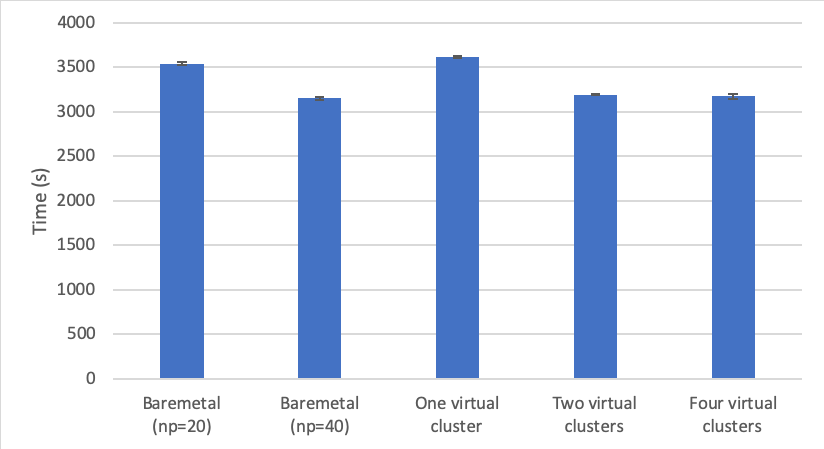
\includegraphics[width=\columnwidth]{Figures/cpu_exe_time}
   \end{center}
   \caption{Comparison of wall clock execution time for a job stream between bare metal and VTC with different CPU over-commitment ratios. Results are average of three runs.}
   \label{fig:cpu_exe_time}
 \end{figure}

Because each node in our testbed has 20 cores, in the first experiment we configured each TORQUE worker with 20 job slots. As reflected in Figure~\ref{fig:cpu_exe_time}, the execution with one virtual cluster is very close to that of bare metal (first column), with only a 2.2 percent overhead. Furthermore, when multiple virtual clusters are used with CPU over-commitment, the execution time is surprisingly shorter, implying an improved throughput despite the virtualization overhead. Through careful analysis, we identified that the throughput improvement can mainly be attributed to increased CPU utilization when more jobs are concurrently scheduled to execute. This has been verified by modifying each TORQUE worker in the bare-metal environment to use 40 job slots, after which the throughput is improved to the same level as the over-committed virtual environment. This can be seen in the second column of Figure~\ref{fig:cpu_exe_time}.

Besides execution time, another performance metric that we monitored is the total CPU utilization across the whole cluster. On the ESXi hypervisor, we used esxtop running on each compute node to sample CPU utilization of all VMs at 5-second intervals, and the results for one, two, and four virtual clusters are shown in Figure~\ref{fig:cpu_utilizations}. With two and four virtual clusters, the decreasing trend at the end is due to job completion. Clearly, CPU utilization is consistent with the job execution times in Figure~\ref{fig:cpu_exe_time}. For example, the lowest CPU utilization case--one virtual cluster--matches the longest job execution time. The higher CPU utilization with two and four virtual clusters is due to resource consolidation brought about by virtualization. That is, when multiple virtual clusters share a physical cluster, the CPU scheduler on each ESXi host has more jobs to schedule and is therefore able to make better scheduling decisions by taking advantage of Hyper-Threading and eliminating idle cycles. At the same time, improved utilization comes with better consistency, where the utilization with two and four virtual clusters is much smoother than in the single-cluster case.

\begin{figure}[!t]
   \begin{center}
       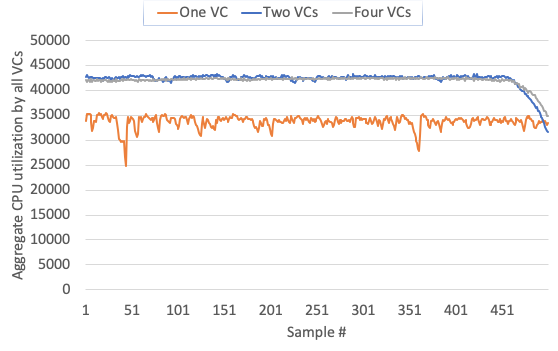
\includegraphics[width=\columnwidth]{Figures/cpu_utilizations}
   \end{center}
   \caption{Aggregate CPU utilization across 16 nodes at 5-seconds intervals.}
   \label{fig:cpu_utilizations}
   \vspace{-0.2in}
 \end{figure}

 In a production cloud environment, an important principle is fairness when multiple tenants are sharing the computing resources. We further examined the per-cluster CPU utilization in the multiple-cluster cases, and the case of four virtual clusters is shown in Figure~\ref{fig:per_cluster_utilization}. It is clear that the ESXi scheduler effectively maintains fairness so that each virtual cluster gets the same amount of CPU resources. The case of two virtual clusters is 
 the same thus not discussed. 


\begin{figure}[!t]
   \begin{center}
       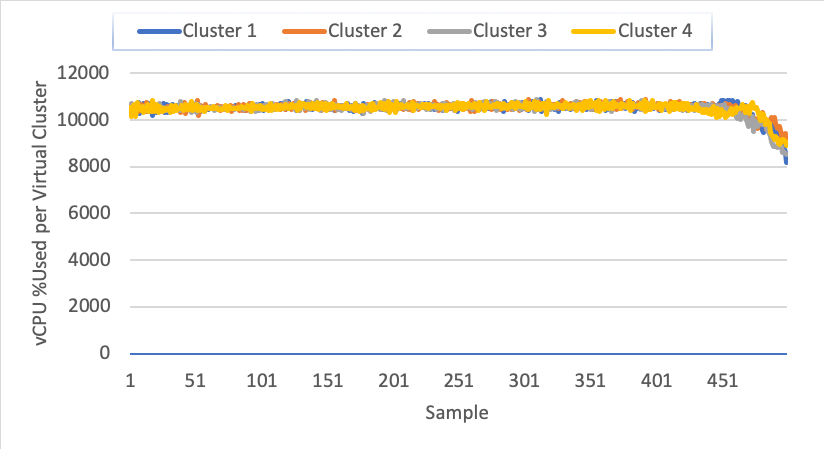
\includegraphics[width=\columnwidth]{Figures/per_cluster_utilization}
   \end{center}
   \caption{Plot of CPU utilization per virtual cluster at 5-seconds intervals for fairness check.}
   \label{fig:per_cluster_utilization}
   \vspace{-0.2in}
 \end{figure}

\subsection{CPU over-commitment with shares}
In addition to the option of equally sharing resources, the proportional, share-based scheduler of the ESXi hypervisor offers a very useful degree of flexibility. This subsection continues the CPU over-commitment study by configuring virtual clusters with different shares, to demonstrate the capability of creating a multi-tenant environment with quality-of-service guarantees. 

With the use of CPU shares, each VM can be given a particular guaranteed share of CPU resources. When there are multiple VMs running on an ESXi host, the ESXi scheduler allocates CPU based on the ratio of shares among all the running VMs. This feature extends to a virtualized HPC cloud. Specifically, each user or group can be given an appropriate share of the physical system when their virtual cluster is allocated. In this experiment, we focus on the case of four virtual clusters and set the shares ratio among the four VMs as 2:1:1:1 on every compute node. The CPU utilization is shown in Figure~\ref{fig:share_utilization}. Clearly, the CPU utilization ratio among the virtual clusters is the same as the specified shares ratio. Another important observation is that the aggregate CPU utilization across 4 virtual clusters is the same as previous no-shares case as depicted in Figure~\ref{fig:cpu_utilizations}.


\begin{figure}[!t]
   \begin{center}
       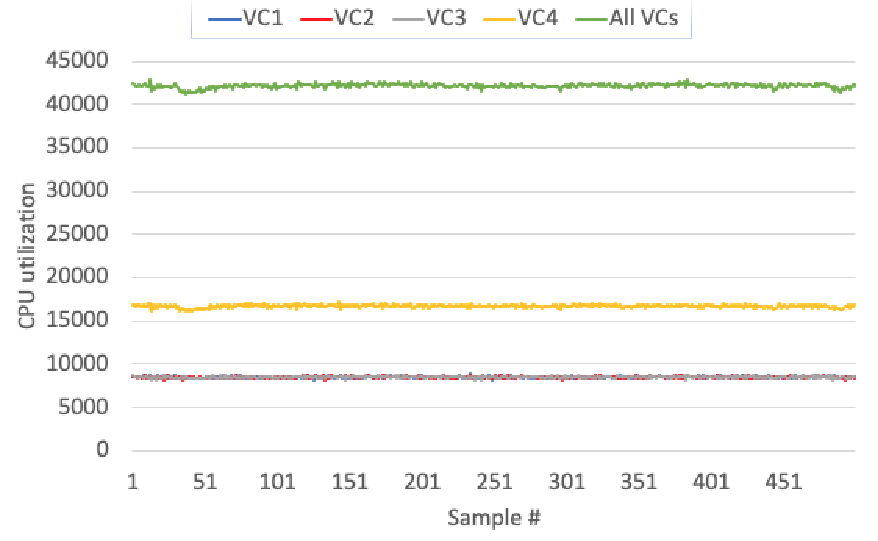
\includegraphics[width=\columnwidth]{Figures/share_utilization}
   \end{center}
   \caption{CPU utilization for four virtual clusters with 2:1:1:1 CPU shares. Utilization is sampled at 5-second intervals.}
   \label{fig:share_utilization}
 \end{figure}

\subsection{CPU + memory over-commitment}
Given that memory over-commitment is more challenging, we only test two virtual clusters with 2X CPU and memory over-commitment. vSphere Dynamic Resource Scheduler (DRS) is used to dynamically control VM migration for load balancing~\cite{infrastructure2006resource}. Considering the VM migration cost, we decided to use four quarter-size VMs to replace the single full-size VM on each node for each tenant. As a result, each tenant in this experiment gets a virtual cluster of 32 VMs across the 8 node cluster. 

To stress the system memory, we added benchmarks from HPCC. For all these HPCC benchmarks, a problem size of 53664 is chosen to have the memory consumption ranging from 16 GB to 22 GB per job instance. All the benchmarks are run with a single threaded process to mimic throughput workloads. 
To model a real HPC tenant, we specify the job arrival time to follow a Gamma distribution based on the study of several production HPC systems~\cite{lublin2003workload}.  
The resulted mean job inter-arrival time is 20.88 seconds
%The Gamma distribution has a shape parameter of 10.23 and scale parameter of 0.49. With those parameters, the mean job inter-arrival time is 10.23 / 0.49 = 20.88 seconds. 
%Also, all job sequences are shuffled to generate randomized job streams. Then, two execution scenarios are designed to represent different workload patterns. 

Two execution scenarios are designed to represent different workload patterns. In the first scenario, 1600 HPCC jobs (memory-intensive) are submitted to the first virtual cluster all at the beginning, while 1500 BioPerf jobs (memory-light) arrive at the second virtual cluster following the above Gamma distribution. The number of jobs are determined to let the two virtual clusters finish at roughly the same time. In the first virtual cluster, all the job slots will be consumed immediately and the jobs will maximize their utilization of the cluster's CPU and memory resources. In the second cluster, CPU and memory load will gradually build up. 
We make the second scenario more demanding by running two HPCC streams of 1600 jobs following the Gamma distribution. 
%Were all job slots being used, the active memory consumption would largely exceed the physical memory capacity. 
It's demanding because, even if each job only consumes 16 GB memory, 64 job instances on each node will require 64 * 16 GB = 1024 GB, which is much larger than the node capacity. It is well understood that ESXi cannot support that kind of memory over-usage. But, it is still worthwhile to explore in the realistic case where jobs randomly come and go, whether DRS can collaborate with ESXi memory reclamation techniques to accommodate this usage pattern. 

In each scenario, we run w/ and w/o DRS and measure two metrics: 1) wall clock time (WCT), i.e., the elapsed time from the start of job submission to the completion of the last job; 2) cumulative job execution time (CJET), i.e., the cumulative sum of all job instances' execution time. 

%The first metric is a measure of the system throughput, and the second metric indicates system efficiency. 
The results in scenario 1 are plotted in Figure~\ref{fig:memory_scenario1}. As the figures suggest, while VTC successfully supported 2X CPU and memory over-commitment regardless of DRS, DRS reduces HPCC's WCT by 11.1\%, which is a great improvement in throughput. 
The reason why DRS doesn't reduce BioPerf's WCT is that BioPerf jobs strictly follow the Gamma distribution in job arrivals.
But as we can see in Figure~\ref{fig:memory_cjet}, DRS reduces BioPerf's CJET by 18.4\%, making room available for more jobs. HPCC's CJET slightly increases with DRS and it indicates that DRS can cause minimal overhead to individual jobs due to telemetry sampling and VM migration. 
%, but increases HPCC CJET by 1.1\%, which is negligible. 
The number of VM migrations in each run is in the range of 30-40. It's interesting to notice that all migrations happened to the BioPerf VMs, which is because BioPerf VMs have smaller memory footprint and are lighter to migrate.

\begin{figure}
     \centering
     \begin{subfigure}[b]{0.45\textwidth}
         \centering
         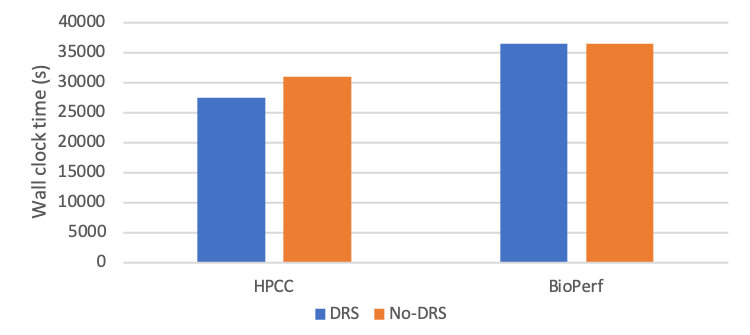
\includegraphics[width=\textwidth]{Figures/memory_wct}
         \caption{Wall clock time}
         \label{fig:memory_wct}
     \end{subfigure}
     \hfill
     \begin{subfigure}[b]{0.45\textwidth}
         \centering
         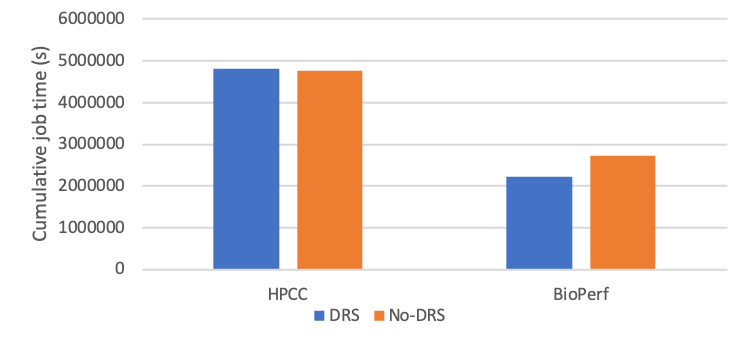
\includegraphics[width=\textwidth]{Figures/memory_cjet}
         \caption{Cumulative job execution time}
         \label{fig:memory_cjet}
     \end{subfigure}
     \caption{Comparison between DRS enabled and DRS disabled for VTC with 2X CPU and memory over-commitment. Workloads are from scenario 1. }
     \label{fig:memory_scenario1}
\end{figure}

As mentioned above, the second scenario is much more demanding because HPCC jobs can potentially consume all the configured VM memory. It's not a surprise the cluster is not able to finish two simultaneous streams of HPCC jobs, regardless of whether DRS is used. The guest OS encountered CPU soft lockup errors when hypervisor swapping occurs and when swapping is not responsive enough. Our analysis identified HPL (one benchmark in the HPCC suite) jobs as the bottleneck. Each HPL job needs more than 3 hours to finish, and once enough HPL instances accumulate on any node, the hypervisor is not able to handle their excessive memory requirements. Therefore, we decided to remove HPL from the job stream. After this change, we see that two HPCC streams can finish when DRS is on. Without DRS, the same failure occurs. Clearly, this demonstrates the effectiveness of DRS in load balancing and mitigating memory pressure. 

Though HPCC VMs are heavier to migrate, on average 67 VM migrations occurred per run, due to the extreme memory stress. Naturally, one may concern that the large number of migrations could introduce jitters to the running workloads. To quantify that, we collect the execution time distribution among all instances for each benchmark. It turns out that the execution time is quite consistent. For example, the histogram for RandomAccess (another benchmark in the HPCC suite) is shown in Figure~\ref{fig:ra_histogram}.

\begin{figure}[!t]
   \begin{center}
       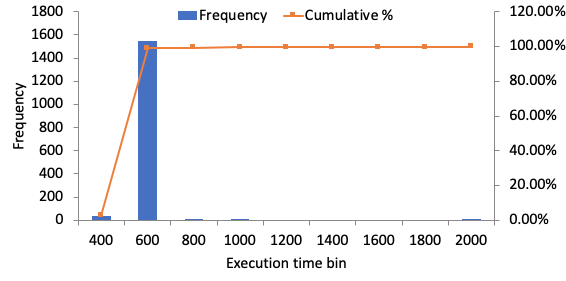
\includegraphics[width=\columnwidth]{Figures/ra_histogram}
   \end{center}
   \caption{Histogram of individual RandomAccess job execution time from both virtual clusters.}
   \label{fig:ra_histogram}
 \end{figure}






\section{Related Work}
\label{sec:related_work}
%Extreme-scale computing presents some unique challenges to fault tolerance as faults are no longer 
%an exceptional event \cite{ferreira_sc_2011}. 
Rollback and recovery is the predominate mechanism to achieve fault
tolerance in current HPC environments. In the most general form, rollback and recovery 
involves the periodic saving of the current system state, with the anticipation that
in the case of a failure, computation can be restarted from the most recently saved state \cite{Elnozahy:02:Survey}. %The identification of an error, before or during a checkpoint,
%requires that the application rollback to the previously completed checkpoint. 
Coordinated checkpointing is a popular approach for
its ease of implementation.
%Specifically, all processes
%coordinate with one another to produce individual states that satisfy the ``happens before"
%communication relationship \cite{chandy_trans_1972}, which is proved to provide a consistent global state.
%Essentially, the algorithm provides a method for all processes involved to stop operation ``at the same
%time" and transfer their system state to a stable storage. 
%The major benefit of coordinated
%checkpointing stems from its simplicity and ease of implementation. 
Its major drawback, however, is the
lack of scalability, as it requires global coordination
\cite{elnozahy_dsc_2004,riesen_sandia_2010}.
%hargrove2006berkeley}.


In uncoordinated checkpointing, processes record their states independently and postpone creating a 
globally consistent view until the recovery phase. The major advantage is the reduced overhead during fault free operation. However, the scheme requires that
each process maintains multiple checkpoints and message logs, necessary to construct a consistent 
state during recovery. It can also suffer the well-known domino effect 
 \cite{randell_domino_effect}. One hybrid approach, known as communication induced 
checkpointing, aims at reducing coordination overhead \cite{alvisi_ftc_1999}. The approach, however, may 
cause processes to store useless states. To address this 
shortcoming, ``forced checkpoints" have been proposed \cite{helary_rds_1997}. This approach, however,  may lead to unpredictable
checkpointing rates. Although well-explored, uncoordinated checkpointing has not been widely adopted
in HPC environments, due to its dependency on applications \cite{guermouche_2011_ipdps}.


One of the largest overheads in any checkpointing process is the time necessary to write the checkpointing 
to stable storage. Incremental checkpointing attempts
to address this by only writing the changes since previous checkpoint \cite{Agarwal:04:Adaptive,elnozahy_1992_manetho,li_trans_1994}. %This
%can be achieved using dirty-bit page flags \cite{plank_ftcs_1994,elnozahy_1992_manetho}. Hash based incremental checkpointing, on the other
%hand, makes use of hashes to detect changes \cite{nam_ftc_1997,Agarwal:04:Adaptive}. 
Another proposed scheme, known as in-memory checkpointing, minimizes the overhead of disk access~\cite{zheng_2004_ftccharm}.
%offloads the checkpointing process to a secondary task and only writes incremental checkpoints \cite{li_trans_1994}.
The main concern of these techniques is the increase in
memory requirement to support the simultaneous execution of the checkpointing and the application. It has been suggested that nodes in extreme-scale systems should be configured with fast local storage~\cite{doe_ascr_exascale_2011}. 
%, which
%improves the performance of checkpointing \cite{doe_ascr_exascale_2011}. 
Multi-level checkpointing, which consists of
writing checkpoints to multiple storage targets, can benefit from such a strategy \cite{Moody:10:SCR}. This,
however, may lead to increased failure rates of individual nodes and complicate the checkpoint writing process.
%Furthermore, it may complicate the checkpoint writing process and requires that the system track the
%current location of all process's checkpoints.


Our work is based on process replication, or state machine replication, which has long been used to provide fault tolerance in distributed and mission critical systems\cite{schneider_1990_tutorial}. %Replication can be used to detect and correct system failures that are otherwise undetectable,
%such as silent data corruption and Byzantine faults \cite{fiala_2012_sdc}. 
Recently, replication has been proposed as a
viable alternative to checkpointing in HPC \cite{ferreira_sc_2011,Cappello:09:Fault,fiala_2012_sdc}. 
In addition, full and partial
replication have also been used to augment existing checkpointing techniques, and to guard
against silent data corruption \cite{stearly_2012_partial,elliott_2012_cpr}.% There are several different implementations of
%replication in the widely used MPI library, each with their different tradeoffs and overheads. The
%overhead can be negligible or up to 70\% depending upon the communication patterns of the
%application \cite{engelmann2011redundant}. %Moreover, replication alone is not enough to guarantee fault tolerance since
%it is possible that all nodes executing a given process could fail simultaneously, thus
%replication is typically paired with some form of checkpointing. 
The most relevant works to ours is redundant multi-threading (RMT) whereby one leading thread of execution is running ahead of trailing threads \cite{reinhardt2000transient,Wadden:2014:RDE:2665671.2665686}. However, our approach is different in that it tunes the execution rates of the leading and trailing threads in a finer grain, in order to achieve a ``parameterized" trade-off between completion time and energy consumption. Further, we take advantage of the idle time during failure recovery and ``leap" the trailing threads to achieve forward progress%, largely improving performance in terms of both completion time and energy consumption. 
. This differs from RMT, of which the ``leaping" of the trailing thread results in extra overhead.
%To the best of our knowledge,
%Lazy Shadowing is the first attempt to explore a state-machine replication based framework
%that achieves a fine-grained tradeoff between time and hardware redundancy while meeting resilience and
%power requirements.


\section{Conclusion}
\label{sec:conclusion}
%Current fault-tolerance approaches rely exclusively on either time or hardware redundancy for recovery. Rollback recovery  exploits time redundancy but can incur significant delay and high energy cost. On the other hand, process replication relies on hardware redundancy and requires a significant increase in resources and  power consumption.

In this paper, we propose Rejuvenating Shadows as a novel power-aware fault tolerance model, which guarantees forward progress, maintains consistent level of resilience, and minimizes implementation complexity and runtime overhead. Empirical experiments demonstrated that the Rejuvenating Shadows model outperforms in-memory checkpointing/restart in both execution time and resource utilization, especially in failure-prone environments.

Leaping induced by failure has proven to be critical in reducing the divergence between a main and its shadow, 
%with respect to workload execution.
%Consequently, the time to recover from subsequent failures is reduced significantly. 
thus reducing the recovery time for subsequent failures. Consequently, the time to recover from a failure increases with failure intervals.  
Based on this observation, a proactive approach is to ``force" leaping when the divergence between a main and its shadow exceeds a specified threshold. 
In our future work, we will further study this approach to determine what behavior triggers forced leaping in order to optimize the average recovery time. 

%we will study forcing the shadDuring experimentation we noticed the problem that recovery time in Rejuvenating Shadows can become substantial when the failure interval is large (Figure~\ref{fig:single_failure}). To deal with this issue, we are studying the idea of ``forced leaping", which borrows the idea from periodic checkpointing and forces a leaping whenever failure has been absent for a long time, in order to reduce the divergence between mains and shadows. Optimal intervals for forced leaping will be explored to balance between runtime overhead and failure recovery overhead. 

%In the future we plan to explore the integration with fault prediction techniques and the viability of dynamic and partial shadowing for platforms where nodes exhibit different ``health" status, e.g., some nodes may be more reliable while others are more likely to fail~\cite{gainaru2012fault}. 
%With this taken into account, we can apply dynamic scheduling of shadows only for mains that are likely to fail, to further reduce the resource requirement. 
%Another future direction is to study complier-assisted program slicing for fault detection. Specifically, slices that are fraction of their mains can run lazily as shadows and provide fault detection capability with reasonable coverage. 





\acknowledgements{Acknowledgements}

This material is based in part upon work supported by the 
National Science Foundation under Grants Number CNS-1252306 and CNS-1253218. 
Any opinions, findings, and conclusions or recommendations expressed in this material are those of the authors and do 
not necessarily reflect the views of the National Science Foundation.

%%%%%%%%%%%%%%%%%%%%%%%%%%%%%%%%%%%%%%%%%%

%%\authorcontributions{Author Contributions}

%%Main text.

%%%%%%%%%%%%%%%%%%%%%%%%%%%%%%%%%%%%%%%%%%

\conflictofinterests{Conflicts of Interest}

%%State any potential conflicts of interest here or 
No conflict of interest to report. 

%=================================================================
% References: Variant A
%=================================================================
% Back Matter (References and Notes)
%----------------------------------------------------------
% Style and layout of the references
%\bibliographystyle{mdpi}
%{\small
%\bibliography{bibliography}}
%
%
%\makeatletter
%\renewcommand\@biblabel[1]{#1. }
%\makeatother
%
%\begin{thebibliography}{999} % if there are less than 10 entries, enter a one digit number
%
%% Reference 1
%\bibitem{ref-journal}
%Lastname, F.; Author, T. The title of the cited article. {\em Journal Abbreviation} {\bf 2008}, {\em 10}, 142-149.
%
%% Reference 2
%\bibitem{ref-book}
%Lastname, F.F.; Author, T. The title of the cited contribution. In {\em The Book Title}; Editor, F., Meditor, A., Eds.; Publishing House: City, Country, 2007; pp. 32-58.
%
%\end{thebibliography}
%
%=================================================================
% References:  Variant B
%=================================================================
% Use the following option to include external BibTeX files:

\bibliographystyle{mdpi}
\bibliography{bibliography}


\end{document}

